\onehalfspacing
The GA is an adaptive search technique derived from the Darwinian theory of natural selection: the individuals having greater fitness will have better chances of survival in a population of organisms. We use this theory as the basis for stress inversion and formulate a minimization problem. Since there are only four unknowns in the reduced stress tensor but a much larger number of fault-slip observations, the inverse problem is over-constrained and a best-fit tensor needs to be determined.

In this optimization problem, the domain of the output parameters is the search space. The initial population, a fixed number of individuals, is sampled randomly from the search space. Analogous to the genetic evolution, the initial population of stress tensors undergoes reproduction, through the natural processes of selection, crossover and mutation, iteratively. We explain each of these processes in the context of stress inversion.

\section{Initialization and Encoding}
We use stochastic sampling to produce an initial population of models, each model set $(\alpha, \beta, \gamma, \phi)$ representing a possible solution to the inverse problem, i.e., a reduced stress tensor. The model parameters are encoded in a binary string, and each model set is referred as a chromosome. The length of the chromosome is dependent upon the number of parameters and the desired resolvability of each parameter.

The four model parameters that describe the reduced stress tensor are each encoded as a 6-bit binary string, making the chromosome 24 bits long (Fig. 2). The mapping of these parameters in real space depends on their ranges defined in the preceding section.

\begin{figure}[h]
\centering
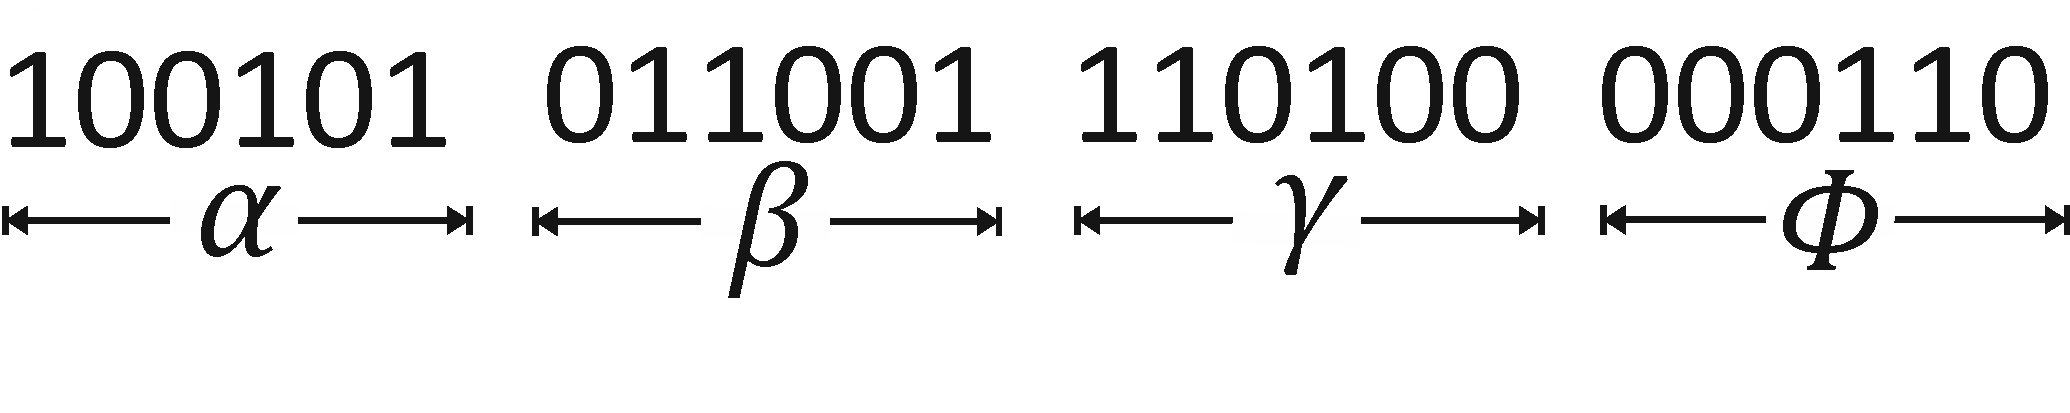
\includegraphics[scale=0.15]{Fig3}
\caption{A chromosome containing 24 binary bits, 6 in each of the four parameters, the three Euler angles ($\alpha, \beta, \gamma$) and the stress-ellipsoid ratio ($\phi$).}
\label{fig3}
\end{figure}

\section{Selection}
The initial population is generated randomly, and each model set is ranked according to the mean misfit function, $\bar{F}$. The next step is to select the best-fit candidates for reproduction. Among a wide range of options that exists for selection, we use the most popular method, the tournament selection. Several tournaments are played between randomly chosen individuals and the winners are selected for mating. Although the misfit criteria decides the winner, the selection of the individuals is essentially stochastic, which prevents the possibility of extinction of a potentially good fit offspring.

\section{Crossover}
Crossover involves exchange of bits between two selected individuals, called `parent models`, to produce two new individuals, called `offspring models`. This is analogous to the exchange of genetic material during reproduction, where the child inherits certain characteristics from both the parents. 
A fixed percentage of previously selected chromosomes, 80\% as a rule of thumb, undergo crossover in the manner described below: (Fig. 4A-C):
\renewcommand{\theenumi}{\roman{enumi}}
\begin{enumerate}
    \item Two crossover sites, e.g., 8th and 15th in Fig. 3A, are randomly selected in the parent chromosomes containing four variables of 6 binary bits each, i.e., 24 bits in total.
    \item The bits lying between the two sites are exchanged between the two parents to produce two offspring (Fig. 4B).
\end{enumerate}

\section{Mutation}
Mutation prevents a rapid convergence of the algorithm to a local optimum. It occurs by flipping a randomly chosen bit in either of the offspring. For example, mutation occurs by flipping the 14th bit from 0 to 1 in the second offspring in Fig. 4B-C. It is carried out with a probability that is low enough to allow the convergence of the solution and high enough so that the solution is not trapped in a local optimum. The probability of mutation is generally taken as 1/(number of bits). Mutation also allows for the possibility of having a better-fit individual, whose characteristics cannot be derived from either parents.

\begin{figure}[h]
\centering
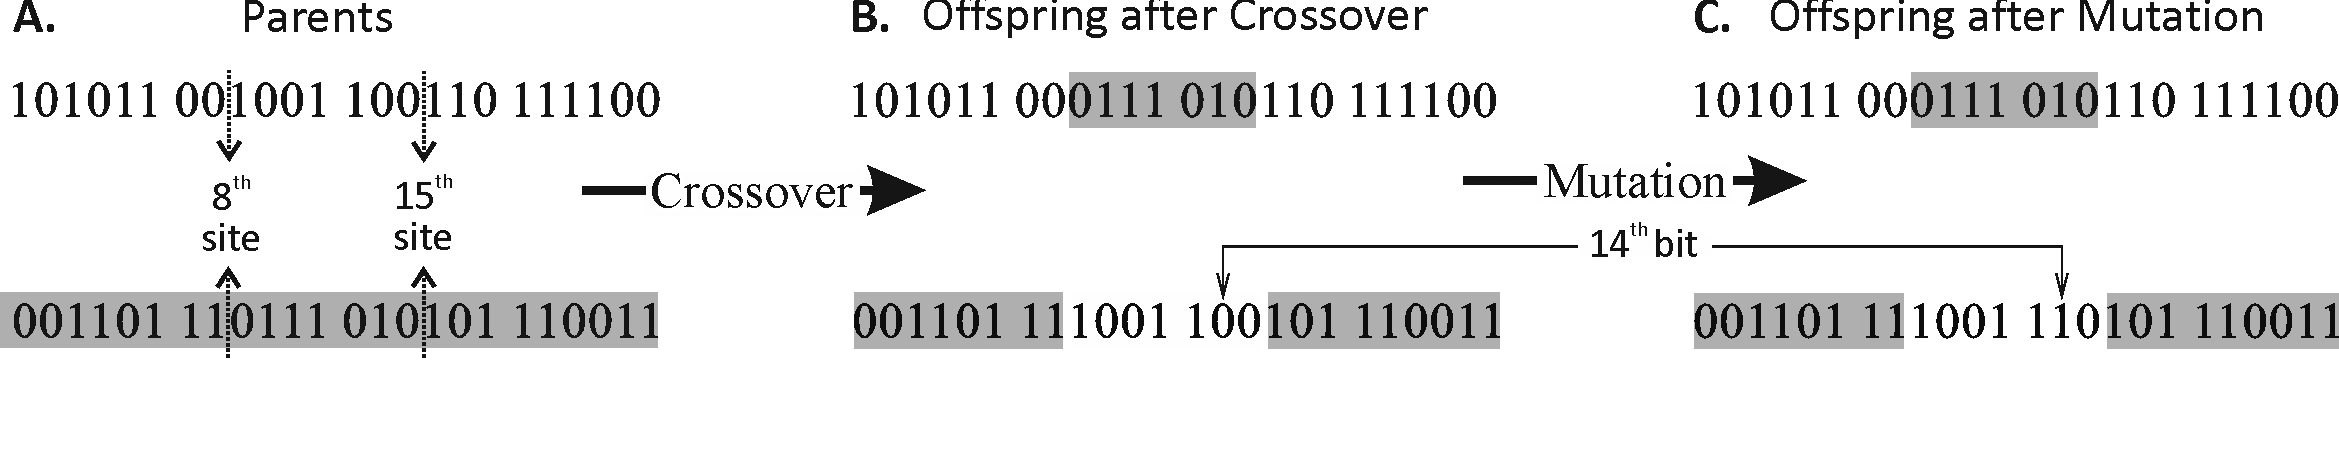
\includegraphics[scale=0.23]{Fig4}
\caption{\textbf{A}: A pair of parents each having 24 binary bits. \textbf{B}: A pair of offspring produced after exchange of bits at two random crossover sites, 8th and 15th, in this case. \textbf{C}: Mutation in the second offspring by flipping of the 14th bit from 0 to 1.}
\label{fig4}
\end{figure}

\section{Termination Criteria}
The pool of the candidates at this stage consist of a fixed percentage of original members and newly created offspring models. The pool is then treated as the next generation that undergoes selection, crossover and mutation again. This process repeats until the mean misfit function stabilizes (Fig. \ref{fig5}).

\begin{figure}[H]
\centering
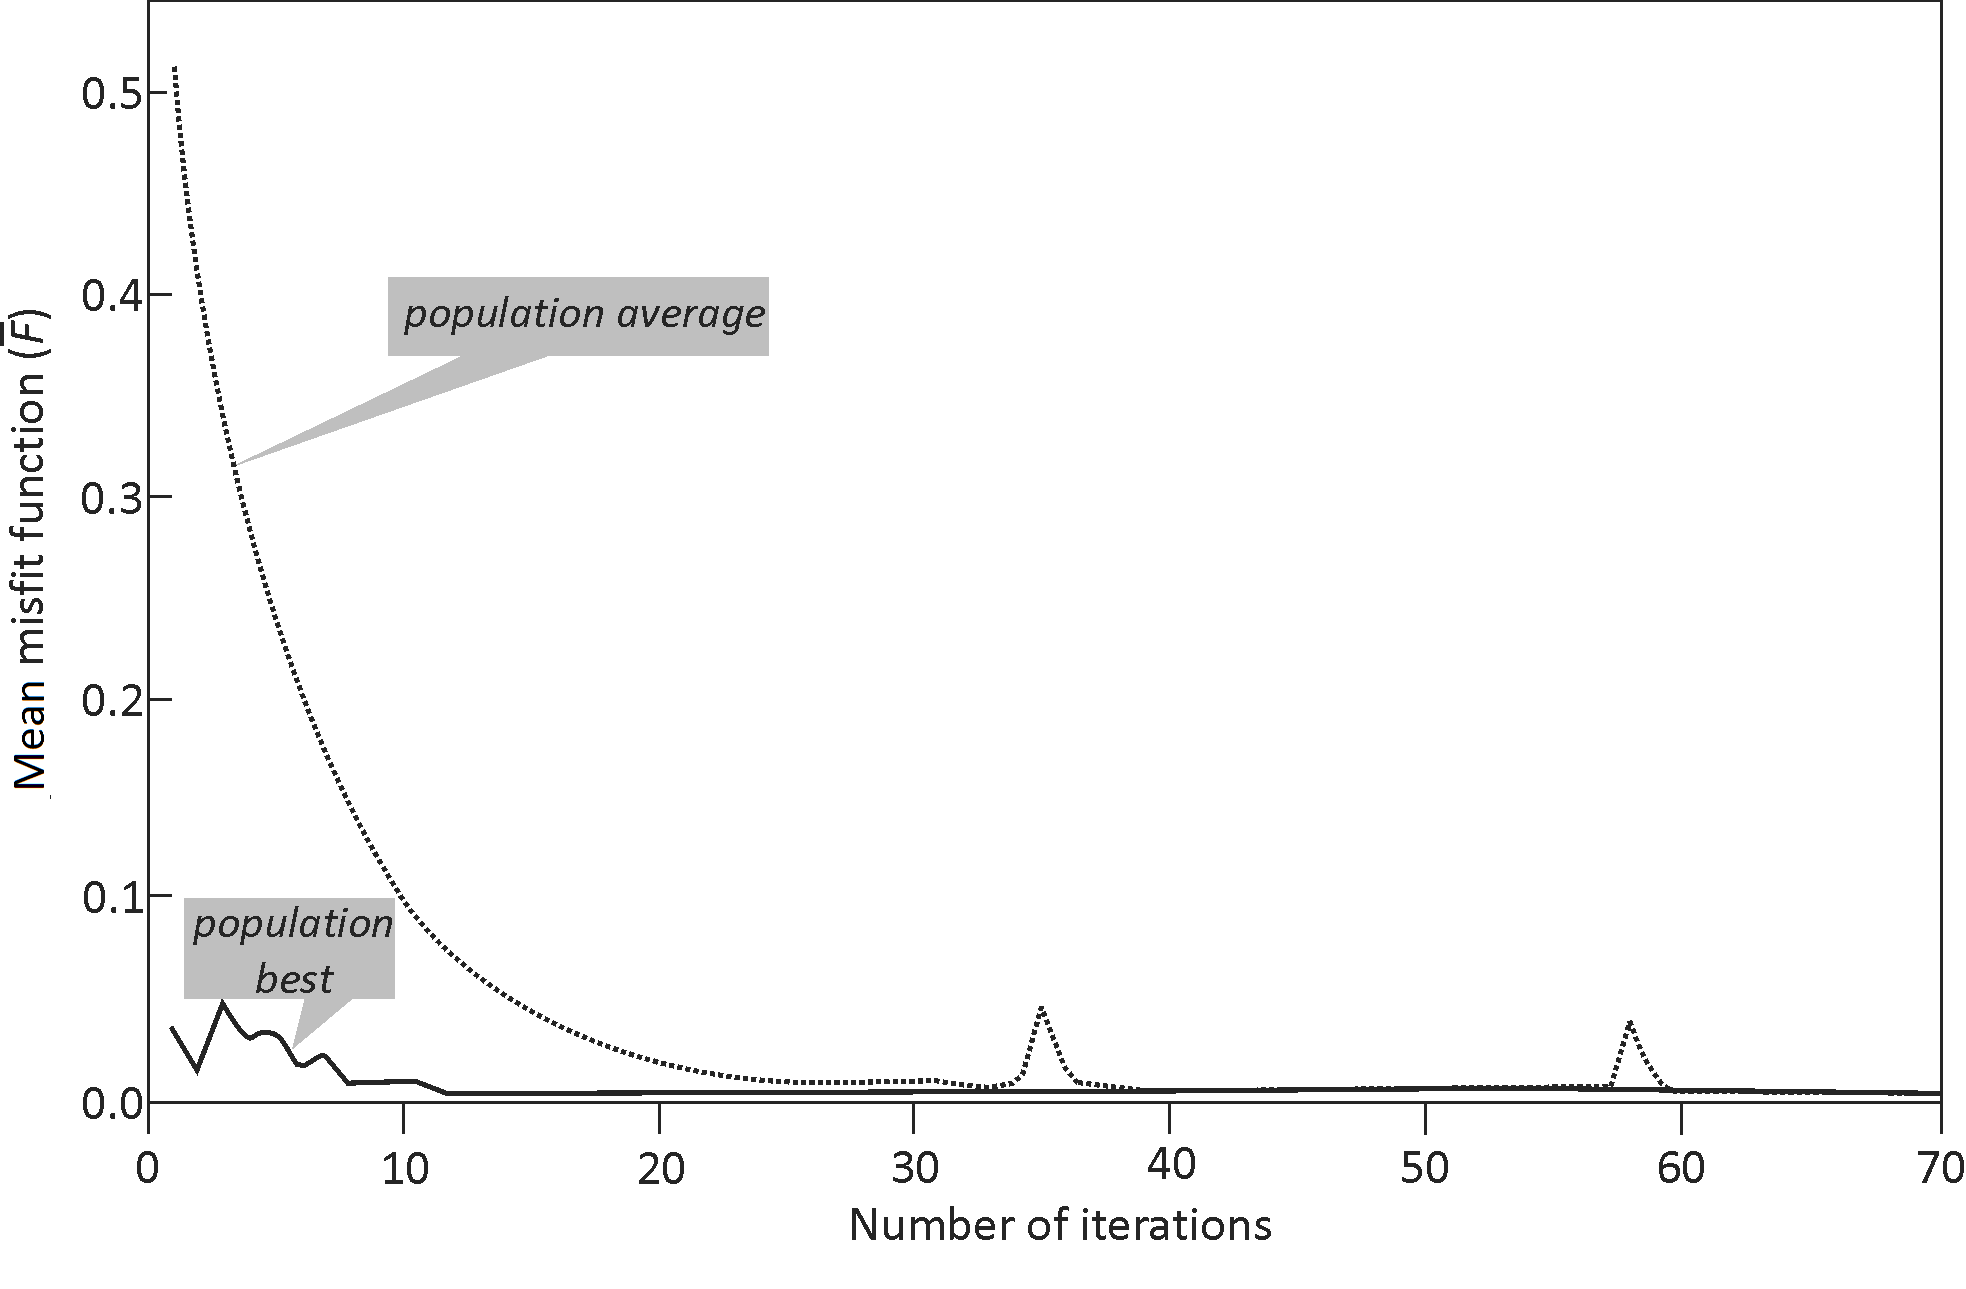
\includegraphics[scale=0.26]{Fig5}
\caption{Convergence curve of the mean misfit function $\bar{F}$ with iterations. Small peaks are caused by chromosomes with mutations.}
\label{fig5}
\end{figure}